\documentclass[a4paper,12pt]{article}
\renewcommand{\familydefault}{\sfdefault}


% Package importing
\usepackage{graphicx}
\usepackage{hyperref}
\hypersetup {
	colorlinks = true,
	linkcolor = cyan,
	urlcolor = cyan,
}
 
 
% Start of document
\begin{document}


% Title
\title{Unity Tool: Dialogue Editor}
\date{}
\maketitle


% Links
\section{Links}
\begin{itemize}
	\item \href{https://assetstore.unity.com/packages/tools/utilities/dialogue-editor-168329}{Asset store}
	\item \href{https://www.youtube.com/playlist?list=PLfRF6lnXtGqjrhzyQhidqMD-shMHGReXi}{Video Tutorial Playlist}
\end{itemize}


% Sections
\section{Tutorial}
\begin{itemize}
	\item \hyperlink{_whatis}{What is Dialogue Editor?}
	\item \hyperlink{_editorwindow}{Editor Window}
	\item \hyperlink{_conversationmanager}{Conversation Manager UI Prefab}
	\item \hyperlink{_triggering}{Triggering a conversation}
	\item \hyperlink{_custominput}{Custom Input}
	\item \hyperlink{_callbacks}{Callbacks}
	\item \hyperlink{_datastructure}{Conversation Datastructure}
\end{itemize}

\newpage


% What is Dialogue Editor
\section{What is Dialogue Editor?}
\hypertarget{_whatis}{}
Dialogue Editor is a Unity tool that allows you to quickly and easily add conversations into your game.
\newline
The tool comes with an editor window that allows you to create and edit conversations.
\newline
This tool also comes with a pre-made, customisable UI prefab so that no UI programming is required. However, if you are comfortable with programming and wish to create your own UI implementation, each conversation can be accessed as a simple data structure.
\newpage


% Editor Window
\section{Editor Window}
\hypertarget{_editorwindow}{}

\subsection{Intro}
Conversations are made up of Speech nodes and Option nodes. Speech nodes represent something a character will say, and Option nodes represent the options available to the player.

\begin{figure}[ht]
\centering
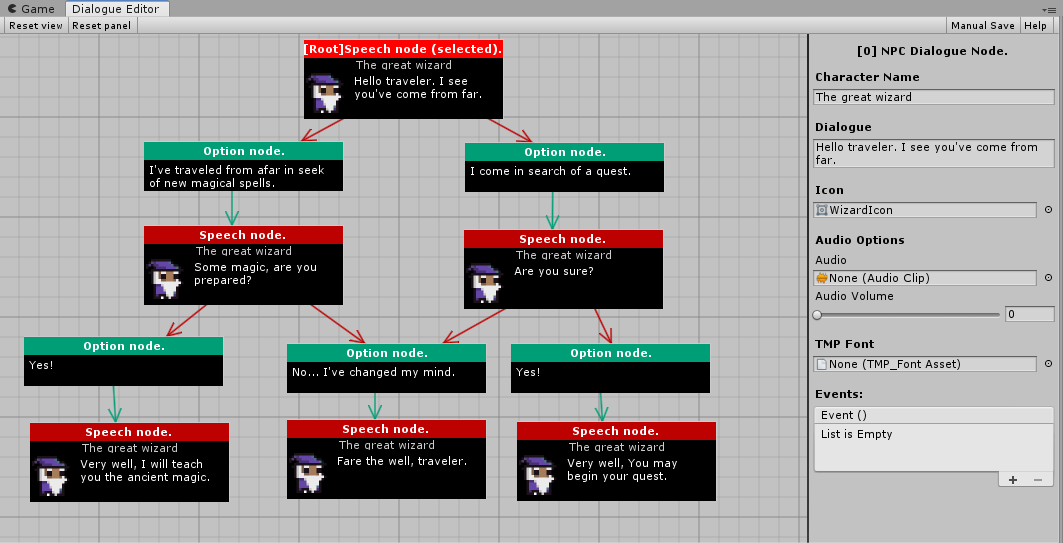
\includegraphics[width=\textwidth,height=\textheight,keepaspectratio]{img/EditorWindowFullConversation.png}
\end{figure}


\subsection{Creating a Conversation Object}
In order to create a conversation, create a new GameObject and add the script NPCConversation. 

\begin{figure}[ht]
\centering
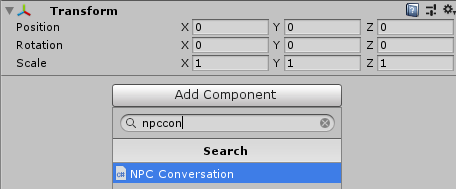
\includegraphics[keepaspectratio]{img/AddNpcConversation.png}
\end{figure}



\subsection{Opening the Editor Window}
In order to open the Editor Window, select Window $\rightarrow$ DialogueEditor. Select a conversation in the hierarchy in order to edit the conversation in the editor window.

\begin{figure}[ht]
\centering
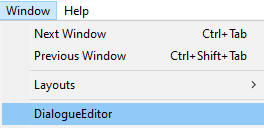
\includegraphics[keepaspectratio]{img/OpenEditorWindow.png}
\end{figure}

\subsection{Speech Nodes}
When you create a new conversation, it will contain a single speech node - this is the beginning of the conversation. 
\newline
Click on a speech node to edit it. A speech node has the following variables:

\begin{itemize}
\setlength\itemsep{1pt}
	\item \textbf{Character Name}: This is the name of the character who is speaking.
	\item \textbf{Dialogue}: This is the speech for the node.
	\item \textbf{Automatically Advance}: This option is available if a speech node leads onto another speech node, or nothing. When this option is selected, the dialogue will automatically continue without the user needing to click anything.
	% sub-list
	\begin{itemize}
		\item \textbf{Display Continue Options}: Should the "Continue" / "End" options still display?
		\item \textbf{Dialogue Time}: How long to wait before the dialogue automatically advances.
	\end{itemize}
	\item \textbf{Icon}: This is the icon of the NPC that will appear next to the speech.
	\item \textbf{Audio}: This is an optional variable, you can play audio with this speech.
	\item \textbf{TMPFont}: This is the TextMeshPro font for this speech. You are able to set fonts on a node-by-node basis.
	\item \textbf{Events}: These are Unity Events that will run when this speech node in a conversation is played.
\end{itemize}

\subsection{Option Nodes}
An Option Node represents an option that a user can select.
\newline
Click on an option node to edit it. An option node has the following variables:

\begin{itemize}
\setlength\itemsep{1pt}
	\item \textbf{Option text}: This is the text for the option.
	\item \textbf{TMP Font}: This is the TextMeshPro font that the option text will use.
\end{itemize}

\subsection{Connecting Nodes}
connecting nodes.

\subsection{Deleting Connections}
deleting connections.

\subsection{Parameters and Conditions}
Parameters and conditions

\newpage


% Conversation Manager 
\section{Conversation Manager}
\hypertarget{_conversationmanager}{}
\newpage

% Triggering a conversation
\section{Triggering a Conversation}
\hypertarget{_triggering}{}
Line.
\newpage

% Custom Input
\section{Custom Input}
\hypertarget{_custominput}{}
\newpage

% Callbacks
\section{Callback}
\hypertarget{_callbacks}{}
\newpage

% Datastructure
\section{Conversation Datastructure}
\hypertarget{_datastructure}{}
\newpage





\end{document}